%%% Please replace what is within each curly bracket with the correct information below. %%%
%%% The first field is already filled in for you.  %%%
\def\ClassName {CS188} % Your course 
\def\NameLast {Manohar}  % Your last name
\def\NameFirst {Jois}  % Your first name
\def\SID{23808180}  % Your SID
\def\Email{m.k.jois@berkeley.edu} % Your pandagrader email
\def\Collaborators{Jesus Garcia} % Any collaborators


%%% Begin 1a %%%
\def\OneA {\textbf{Put your answer to 1a here:} 
\begin{align*}
P(A=+m|B=+m,C=+m) &= \frac{P(B=+m|A=+m)P(C=+m|A=+m)P(A=+m)}{P(B=+m,C=+m)}\\
&= \frac{0.9\times 0.9\times 0.5}{P(B=+m,C=+m|A=+m)P(B=+m,C=+m|A=-m)}\\
&= \frac{0.81 \times 0.5}{0.5\times 0.81 + 0.5 \times 0.01}\\
&= 81/82
\end{align*} 
}
%%% End 1a %%%

%%% Begin 1b %%%
\def\OneB {\textbf{Put your answer to 1b here:} 
\begin{align*}
P(D=+m|A=+m) &= P(D=+m|B=+m)P(B=+m|A=+m) + P(D=+m|B=-m)P(B=-m|A=+m)\\
&= 0.9 \times 0.9 + 0.1 \times 0.1\\
&= 0.82
\end{align*}
}
%%% End 1b %%%

%%% Begin 1c %%%
\def\OneC {\textbf{Put your answer to 1c here:} 
\begin{align*}
P(D=+m) &= 0.5 \text{ (by symmetry)}\\
EU(march) &= (+1)\times P(A=+m|D=+m) + (-1)\times P(A=-m|D=+m)\\
&= \frac{0.82\times 0.5}{0.5} - \frac{0.18\times 0.5}{0.5}\\
&= 0.64\\
EU(stay) &= (+1)\times P(A=-m|D=+m) + (-1)\times P(A=+m|D=+m)\\
&= -0.64 \text{ (by symmetry)}\\
MEU &= 0.64
\end{align*}
}
%%% End 1c %%%

%%% Begin 1d %%%
\def\OneD {\textbf{Put your answer to 1d here:} 
\begin{align*}
EU(\text{march}|A=+m) &= 1\\
EU(\text{stay}|A=+m) &= -1\\
EU(\text{march}|A=-m) &= -1\\
EU(\text{stay}|A=-m) &= 1\\
MEU(|A) &= (1)P(A=+m) + (1)P(A=-m)\\
&= 1\\
VPI(A|D=+m) &= 1-0.64\\
&= 0.36
\end{align*}
}
%%% End 1d %%%

%%% Begin 1e %%%
\def\OneE {\textbf{Put your answer to 1e here:} 
\begin{align*}
P(A=+m|D=+m,B=-m) &= 0.1 \text{ (by intuition)}\\
P(A=-m|D=+m,B=-m) &= 0.9 \text{ (by intuition)}\\
EU(march) &= 0.1 - 0.9\\
&= -0.8\\
EU(stay) &= 0.9 - 0.1\\
&= 0.8\\
VPI(A|D=+m,B=-m) &= 1-0.8\\
&= 0.2
\end{align*}
}
%%% End 1e %%%

%%% Begin 2a %%%
%%% Fill in an optimal policy: \actionNorth \actionSouth \actionEast \actionWest \actionStay . Put within curly brackets below.
%%% 1st row
\def\polZeroZero{\actionStay}
\def\polZeroOne{\actionSouth}
\def\polZeroTwo{\actionSouth}
%%% 2nd row
\def\polOneZero{\actionWest}
\def\polOneOne{\actionSouth}
\def\polOneTwo{\actionWest}
%%% 3rd row
\def\polTwoZero{\actionWest}
\def\polTwoOne{\actionSouth}
\def\polTwoTwo{\actionWest}

%%% Fill in the value function: Fill in the value of each state within the curly brackets below.

%%% 1st column
\def\vZeroZero{10}
\def\vZeroOne{9}
\def\vZeroTwo{8}
%%% 2nd column
\def\vOneZero{9}
\def\vOneOne{8}
\def\vOneTwo{7}
%%% 3rd column
\def\vTwoZero{8}
\def\vTwoOne{7}
\def\vTwoTwo{6}
%%% End 2a %%%

%%% Begin 2b %%%
\def\TwoBi {9}
\def\TwoBii {6}
%%% End 2b %%%

%%% Begin 2c %%%
\def\TwoCi {false} % type true or false
\def\TwoCii {5}

%%% End 2c %%%

%%% Begin 2d %%%
\def\TwoD {10} 

%%% End 2d %%%

%%% Begin 2e %%%
\def\TwoE {10}
%%% End 2e %%%

%%% For 3a and 3b, replace \mcqb with \mcqs for the correct answer.
%%% Begin 3a %%%
\def\ThreeA{
  \mcqb $J^*(s) = \min_{a} \sum_{s'} {[C(s,a,s') + \gamma \max_{a'}{T(s,a',s')*J^*(s')}]}$ \\[1mm]
  \mcqb $J^*(s) = \min_{s'} \sum_{a} {T(s,a,s')[C(s,a,s') + \gamma*J^*(s')]}$ \\[1mm]
  \mcqb $J^*(s) = \min_{a} \sum_{s'} {T(s,a,s')[C(s,a,s') + \gamma * \max_{s'}{J^*(s')}]}$ \\[1mm]
  \mcqb $J^*(s) = \min_{s'} \sum_{a} {T(s,a,s')[C(s,a,s') + \gamma * \max_{s'}{J^*(s')}]}$ \\[1mm]
  \framebox[9cm][l]{\mcqb $J^*(s) = \min_{a} \sum_{s'} {T(s,a,s')[C(s,a,s') + \gamma*J^*(s')]}$} \\[1mm]
  \mcqb $J^*(s) = \min_{s'} \sum_{a} {[C(s,a,s') + \gamma * {J^*(s')}]}$
}
%%% End 3a %%%

%%% Begin 3b %%%
\def\ThreeB{
  \mcqb $J^*(s) = \min_{a} \max_{s'} {T(s,a,s')[C(s,a,s') + \gamma*J^*(s')]}$ \\[1mm]
  \mcqb $J^*(s) = \min_{s'} \sum_{a} {T(s,a,s')[\max_{s'} C(s,a,s') + \gamma*J^*(s')]}$ \\[1mm]
  \mcqb $J^*(s) = \min_{a} \min_{s'} {[C(s,a,s') + \gamma* \max_{s'}J^*(s')]}$ \\[1mm]
  \framebox[8cm][l]{\mcqb $J^*(s) = \min_{a} \max_{s'} {[C(s,a,s') + \gamma*J^*(s')]}$} \\[1mm]
  \mcqb $J^*(s) = \min_{s'} \sum_{a} {T(s,a,s')[\max_{s'} C(s,a,s') + \gamma*\max_{s'}J^*(s')]}$ \\[1mm]
  \mcqb $J^*(s) = \min_{a} \min_{s'} {T(s,a,s')[C(s,a,s') + \gamma*J^*(s')]}$
}
%%% End 3b %%%

%%% Begin 4a %%%
\def\FourA {\textbf{Put your answer to 4a here:} \\
M$\leftarrow$------B(action)---\\
$\mid$\hspace{1.4cm}$\mid$\hspace{1.5cm}$\mid$\\
$\mid$\hspace{1.4cm}$\mid$\hspace{1.5cm}$\mid$\\
$\downarrow$\hspace{1.3cm}$\mid$\hspace{1.5cm}$\downarrow$\\
P$\leftarrow$---------\hspace{1.4cm}U(utility)\\
$\mid$\hspace{3cm}$\uparrow$\\
$\mid$\hspace{3cm}$\mid$\\
---------------------------
}
%%% End 4a %%%

%%% Begin 4b %%%
\def\FourB {\textbf{Put your answer to 4b here:} 
\begin{align*}
P(+p|+b) &= 0.9(1.0) + 0.1(0.5) = 0.95\\
P(-p|+b) &= 0.9(0.0) + 0.1(0.5) = 0.05\\
P(+p|-b) &= 0.7(0.7) + 0.3(0.2) = 0.55\\
P(-p|-b) &= 0.7(0.3) + 0.3(0.8) = 0.45\\
EU(+b) &= 0.95(2000-100) + 0.05(0-100) = 1800\\
EU(-b) &= 0.55(2000+0) + 0.45(0+0) = 1100
\end{align*}
}
%%% End 4b %%%

%%% Begin 4c %%%
\def\FourC {true} % type true or false
%%% End 4c %%%

%%% Begin 5 %%%
\def\FiveA {\textbf{Put your answer to 5a here:}
\begin{align*}
U_A(s) &= \max_{a: s\rightarrow s'}{(R(s)+\min_{a': s'\rightarrow s''}{(-R(s') + U_A(s''))})}\\
U_B(s) &= \min_{a: s\rightarrow s'}{(-R(s)+\max_{a': s'\rightarrow s''}{(R(s') + U_B(s''))})}
\end{align*}
}
%%% End 5 %%%

%%%%%%%%%%%%%%%%%%%%%% DO NOT CHANGE ANYTHING BELOW THIS LINE %%%%%%%%%%%%%%%%%%%%%%%%%
% \def \showSolutions {} 
\documentclass[twoside]{article}

\usepackage{class}
%\usepackage{verbatim}
\usepackage{fancyhdr}
\usepackage{booktabs}
\usepackage{setspace}
\usepackage{amsmath,mathrsfs}
\usepackage{multicol}
\usepackage{amssymb}
\usepackage{tikz}
\usetikzlibrary{matrix}
\usepackage{graphicx}
\usepackage{subfig}
\usepackage{array}
\usepackage{xcolor}
\usepackage{float}
\usepackage{enumitem}
\usepackage{mathcomp}
\usepackage{tabularx}
\usepackage{wasysym}
\usepackage{pbox}
\usetikzlibrary{bayesnet}

% Bubbles for multiple choice questions
\newcommand{\mcqbubble}{\bigcirc}
\newcommand{\mcqbubblefill}{\Large\newmoon}

% shorthand
\newcommand{\mcqb}{$\bigcirc$\ \ }
\newcommand{\mcqs}{\solution{\mcqb}{$\Large\newmoon$\ \ }}

% pruning
\newcommand{\prune}{\includegraphics[width=0.2in]{figures/red_x}}
% title is Written HW8
\title{Written HW8}
\begin{document}
\thispagestyle{empty}
\maketitle


\smallskip
\smallskip
\textbf{INSTRUCTIONS}

\begin{itemize}
\item \textbf{Due:} Monday, November 3rd, 2014 11:59 PM
\item \textbf{Policy:} Can be solved in groups (acknowledge collaborators) but must
be written up individually. However, we strongly encourage you to first work alone for about 30 minutes total in order to simulate an exam environment.  Late homework will not be accepted.
\item \textbf{Format:}
You must solve the questions on this handout (either through a pdf annotator, or by printing, then scanning; we recommend the latter to match exam setting). Alternatively, you can typeset a pdf on your own that has answers appearing in the same space (check edx/piazza for latex templating files and instructions).
\textbf{Make sure that your answers (typed or handwritten) are within the
dedicated regions for each question/part.  If you do not follow this format, we may deduct points.}

\item \textbf{How to submit:}  Go to www.pandagrader.com. Log in and click on the
class CS188 Fall 2014. Click on the submission titled Written HW 8 and upload your pdf containing your answers. If this is your first time using pandagrader, you will have to set your password before logging in the first time.  To do so, click on "Forgot your password" on the login page, and enter your email address on file with the registrar's office (usually your @berkeley.edu email address). You will then receive an email with a link to reset your password.

\end{itemize}


\begin{center}
\begin{tabular}{|r|c|}
\hline
\begin{minipage}{3cm}~\\Last Name~\\~\\\end{minipage} & \begin{minipage}[c][1cm][c]{8cm} ~ \NameLast \end{minipage}  \\
\hline
\begin{minipage}{3cm}~\\First Name~\\~\\\end{minipage} & \NameFirst \\
\hline
\begin{minipage}{3cm}~\\SID~\\~\\\end{minipage} & \SID \\
\hline
\begin{minipage}{3cm}~\\Email~\\~\\\end{minipage} & \Email \\
\hline
\begin{minipage}{3cm}~\\Collaborators~\\~\\\end{minipage} & \Collaborators \\
\hline

\end{tabular}
\end{center}

\newpage
\begin{problem}[]{Occupy Cal}

You are at Occupy Cal, and the leaders of the protest are deciding whether or not to march on California Hall. The decision is made centrally and communicated to the occupiers via the ``human microphone''; that is, those who hear the information repeat it so that it propagates outward from the center. This scenario is modeled by the following Bayes net:

\vspace{2mm}
\begin{figure}[htp]
\centering
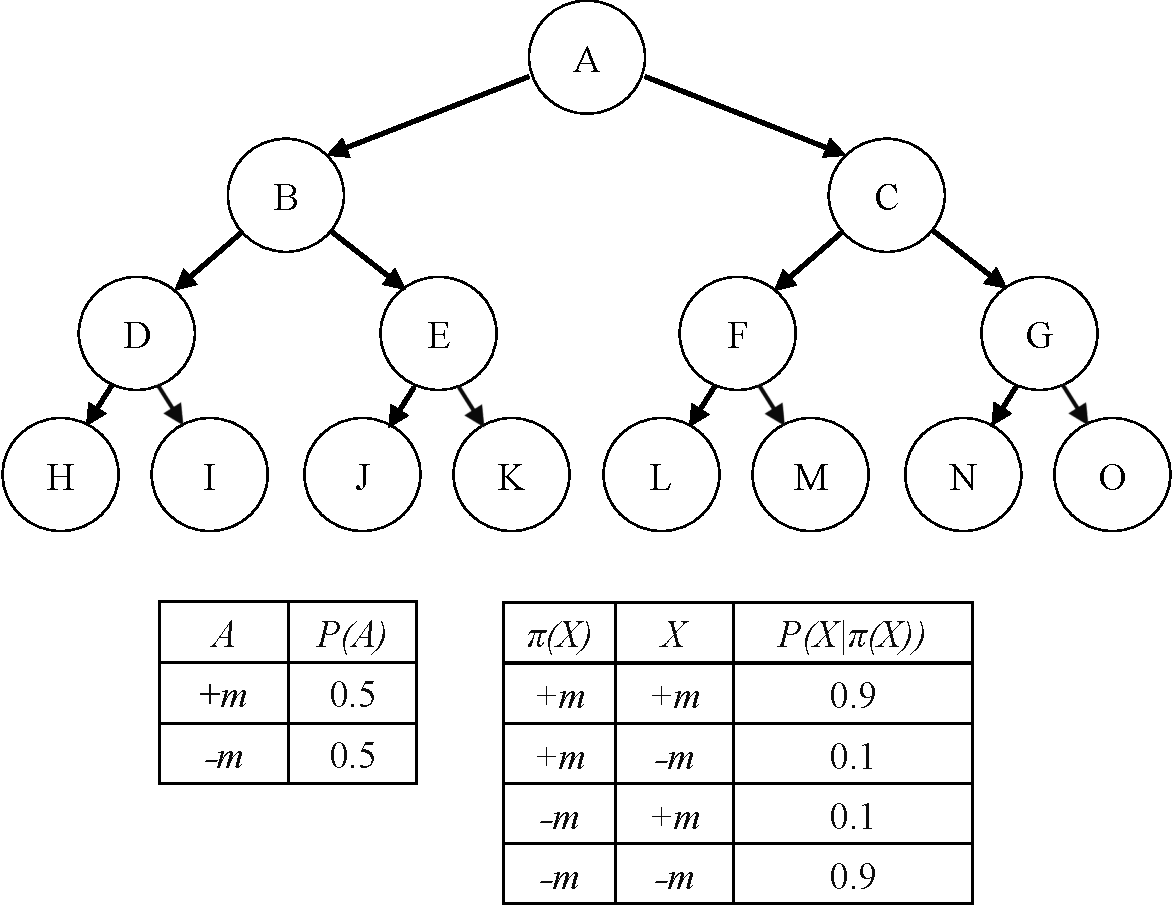
\includegraphics[width=105mm]{figures/tree-labeled-tables-crop.pdf}
\end{figure}
\vspace{2mm}

Each random variable represents whether a given group of protestors hears instructions to march ($+m$) or not ($-m$). The decision is made at $A$, and both outcomes are equally likely. The protestors at each node relay what they hear to their two child nodes, but due to the noise, there is some chance that the information will be misheard. Each node except $A$ takes the same value as its parent with probability 0.9, and the opposite value with probability 0.1, as in the conditional probability tables shown.

\begin{question}[4] Compute the probability that node $A$ sent the order to march ($A = +m$) given that both $B$ and $C$ receive the order to march ($B=+m$, $C=+m$). \\
\fbox{\begin{minipage}[t][4cm][t]{17cm}
\OneA
\end{minipage}}
\end{question}

\begin{question}[4] Compute the probability that $D$ receives the order $+m$ given that $A$ sent the order $+m$. \\
\fbox{\begin{minipage}[t][4cm][t]{17cm}
\OneB
\end{minipage}}
\end{question}

You are at node $D$, and you know what orders have been heard at node $D$. Given your orders, you may either decide to march (\emph{march}) or stay put (\emph{stay}). (Note that these actions are distinct from the orders $+m$ or $-m$ that you hear and pass on. The variables in the Bayes net and their conditional distributions still behave exactly as above.) If you decide to take the action corresponding to the decision that was actually made at $A$ (not necessarily corresponding to your orders!), you receive a reward of $+1$, but if you take the opposite action, you receive a reward of $-1$. \\

\begin{question}[4] Given that you have received the order $+m$, what is the expected utility of your optimal action? (Hint: your answer to part (b) may come in handy.) \\
\fbox{\begin{minipage}[t][5cm][t]{17cm}
\OneC
\end{minipage}}
\end{question}

Now suppose that you can have your friends text you what orders they have received. (Hint: for the following two parts, you should not need to do much computation due to symmetry properties and intuition.)

\begin{question}[4] Compute the VPI of $A$ given that $D = +m$. \\
\fbox{\begin{minipage}[t][5cm][t]{17cm}
\OneD
\end{minipage}}
\end{question}

\begin{question}[4] Compute the VPI of $A$ given that $D = +m$ and $B = -m$. \\
\fbox{\begin{minipage}[t][5cm][t]{17cm}
\OneE
\end{minipage}}
\end{question}

\end{problem}
\newpage
\q{30}{Neural Networks}

In this problem, you are given a simple network that uses the simple linear function $g(x) = mx + b$ (where $m$ and $b$ values are fixed) as the activation function (rather than, for example,  a sigmoid function). You will need to write the $L_2$ norm (squared) loss function, the partial derivative of the loss function, and the gradient descent update rule for certain weights.

\textbf{Single Neuron Example}

We have given you the answers for the loss function, partial derivative, and weight update rule for the following single neuron example. This example should help you understand how to structure your answers to the questions about the slightly more complex network on the following page.

\begin{figure}[h]
\centering
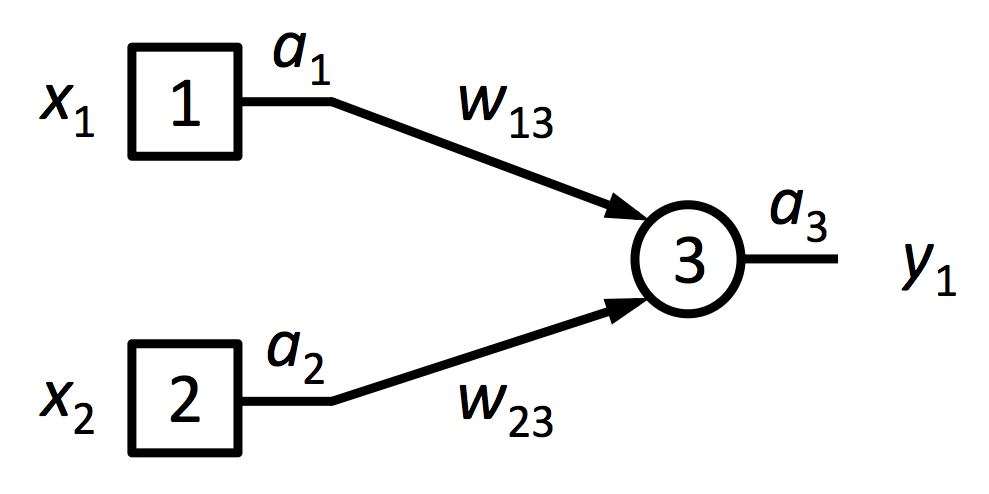
\includegraphics[width=0.25\linewidth]{figs/NN_1.png}
\end{figure}
\begin{flalign*}
a_1 &= x_1 &\\
a_2 &= x_2 &\\
a_3 &= m(w_{13}a_1+w_{23}a_2) + b &
\end{flalign*}
\textbf{Loss function}
\begin{flalign*}
Loss(\boldsymbol{w}) &= ||\boldsymbol{y}-\boldsymbol{h_w}(\boldsymbol{x})||_2^2 &\\
&= (y_1 - a_3)^2 &\\
&= (y_1 - m(w_{13}a_1+w_{23}a_2) - b)^2 &\\
&= (y_1 - m(w_{13}x_1+w_{23}x_2) - b)^2 &
\end{flalign*}
\textbf{Loss partial derivative}
\begin{flalign*}
\frac{\partial }{\partial w_{13}}Loss(\boldsymbol{w}) &= -2(y_1 - a_3) \frac{\partial a_3}{\partial w_{13}} &\\
&= -2(y_1 - a_3)ma_1 &\\
&= -2(y_1 - m(w_{13}x_1+w_{23}x_2) - b)mx_1 &
\end{flalign*}
\textbf{Weight update rule}
\begin{flalign*}
w_{13} &\leftarrow w_{13} - \alpha \frac{\partial }{\partial w_{13}} Loss(\boldsymbol{w})&\\
&= w_{13} + \alpha 2(y_1 - m(w_{13}x_1+w_{23}x_2) - b)mx_1 &
\end{flalign*}

(Question continued on next page)

\newpage
\textbf{Simple Neural Network with Linear Activation Function}

Given the following neural network (again, using the simple linear activation function $g(x) = mx + b$):

\begin{figure}[h]
\centering
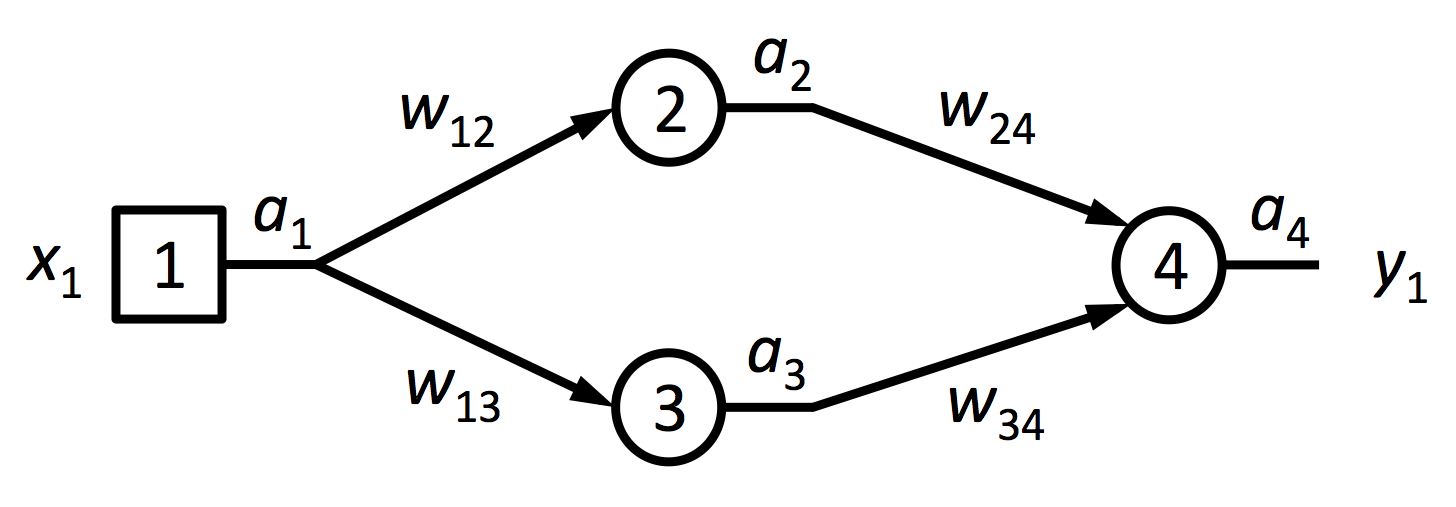
\includegraphics[width=0.4\linewidth]{figs/NN_2.png}
\end{figure}

\begin{question}{[5 pts]}
Write the loss function, $Loss(\boldsymbol{w})$, in terms of $x_1$, $y_1$, $w_{12}$, $w_{13}$, $w_{24}$, $w_{34}$, $m$, and $b$.

\begin{minipage}{\textwidth}
    \solution{} {\begin{align*}
    Loss(\boldsymbol{w}) &= (y_1-a_4)^2\\
    &= (y_1-m(w_{24}a_2+w_{34}a_3)-b)^2\\
    &= (y_1-m(w_{24}(mw_{12}a_1+b)+w_{34}(mw_{13}a_1+b))-b)^2\\
    &= (y_1-m^2w_{12}w_{24}x_1-mw_{24}b-m^2w_{13}w_{34}x_1-mw_{34}b-b)^2
    \end{align*}
    }
\end{minipage}

\end{question}

\begin{question}{[5 pts]}
Write the derivative of the loss function with respect to $w_{24}$, $\frac{\partial}{\partial w_{24}} Loss(\boldsymbol{w})$, in terms of $x_1$, $y_1$, $w_{12}$, $w_{13}$, $w_{24}$, $w_{34}$, $m$, and $b$.

\begin{minipage}{\textwidth}
    \solution{} {\begin{align*}
    \frac{\partial}{\partial w_{24}}Loss(\boldsymbol{w}) &= -2(y_1-a_4)\frac{\partial a_4}{\partial w_{24}}\\
    &= -2ma_2(y_1-a_4)\\
    &= -2m(mw_{12}x_1+b)(y_1-m^2w_{12}w_{24}x_1-mw_{24}b-m^2w_{13}w_{34}x_1-mw_{34}b-b)
    \end{align*}
    }
\end{minipage}

\end{question}

\begin{question}{[2 pts]}
Write the gradient descent update rule for $w_{24}$ with step size $\alpha$ in terms of $\alpha$ $x_1$, $y_1$, $w_{12}$, $w_{13}$, $w_{24}$, $w_{34}$, $m$, and $b$.

\begin{minipage}{\textwidth}
    \solution{} {\begin{align*}
    w_{24} &\leftarrow w_{24}-\alpha\frac{\partial}{\partial w_{24}} Loss(\boldsymbol{w})\\
    &= w_{24}+2\alpha m(mw_{12}x_1+b)(y_1-m^2w_{12}w_{24}x_1-mw_{24}b-m^2w_{13}w_{34}x_1-mw_{34}b-b)
    \end{align*}
    }
\end{minipage}

\end{question}

\begin{question}{[5 pts]}
Write the derivative of the loss function with respect to $w_{12}$, $\frac{\partial}{\partial w_{12}} Loss(\boldsymbol{w})$, in terms of $x_1$, $y_1$, $w_{12}$, $w_{13}$, $w_{24}$, $w_{34}$, $m$, and $b$.

\begin{minipage}{\textwidth}
    \solution{} {\begin{align*}
    \frac{\partial}{\partial w_{12}}Loss(\boldsymbol{w}) &= -2(y_1-a_4)\frac{\partial a_4}{\partial w_{12}}\\
    &= -2(y_1-a_4)(mw_{24}\frac{\partial a_2}{\partial w_{12}}+mw_{34}\frac{\partial a_3}{\partial w_{12}})\\
    &= -2(y_1-a_4)(mx_1+0)\\
    &= -2mx_1(y_1-m^2w_{12}w_{24}x_1-mw_{24}b-m^2w_{13}w_{34}x_1-mw_{34}b-b)
    \end{align*}
    }
\end{minipage}

\end{question}

\begin{question}{[2 pts]}
Write the gradient descent update rule for $w_{12}$ with step size $\alpha$ in terms of $\alpha$ $x_1$, $y_1$, $w_{12}$, $w_{13}$, $w_{24}$, $w_{34}$, $m$, and $b$.

\begin{minipage}{\textwidth}
    \solution{} {\begin{align*}
    w_{12} &\leftarrow w_{12}-\alpha\frac{\partial}{\partial w_{12}} Loss(\boldsymbol{w})\\
    &= w_{12}+2\alpha mx_1(y_1-m^2w_{12}w_{24}x_1-mw_{24}b-m^2w_{13}w_{34}x_1-mw_{34}b-b)
    \end{align*}
    }
\end{minipage}
\end{question}

\newpage

\begin{question}{[3 pts]}
Because this network has a linear activation function, there is an equivalent network that has no hidden layers. 1) Draw a new (very simple) network that has no hidden layers but computes exactly the same function. 2) Write the new weight explicitly in terms of the $w_{12}$, $w_{13}$, $w_{24}$, $w_{34}$, $m$, and $b$. 3) You will need to adjust the linear activation function, $g_2(x) = m_2x + b_2$. Write the new $m_2$ and $b_2$ values in terms of $w_{12}$, $w_{13}$, $w_{24}$, $w_{34}$, $m$, and $b$.

\begin{minipage}{\textwidth}
    \solution{} {\begin{verbatim}
    x1 (1) a1 -----------> (2) a2', y1
                   w'
    \end{verbatim}
    \begin{align*}
    a2' &= a4\\
    &= m^2w_{12}w_{24}x_1+mw_{24}b+m^2w_{13}w_{34}x_1+mw_{34}b+b\\
    &= m^2(w_{12}w_{24}+w_{13}w_{34})x_1 + (mw_{24}b+mw_{34}b+b)\\
    w' &= w_{12}w_{24}+w_{13}w_{34}\\
    m_2 &= m^2\\
    b_2 &= mw_{24}b+mw_{34}b+b
    \end{align*}
    }
\end{minipage}
\end{question}

\textbf{General Neural Network with Linear Activation Function}

\vspace{3mm}
Consider a new neural network with $n$ input nodes, $n$ output nodes, one hidden layer with $h$ nodes, and the linear activation function $g(x) = mx + b$ at each hidden and output node. The nodes between each layer are fully connected with weights $w_{ij}$ from the $i$-th input node to the $j$-th hidden node and weights $w_{jk}$ from the $j$-th hidden node to the $k$-th output node.

\vspace{3mm}
\begin{question}{[5 pts]}
Because this general network has a linear activation function, there is an equivalent network that has no hidden layers that computes exactly the same function. 1) Write an equation for the weight $w_{ik}$ from the $i$-th input node to the $k$-th output node explicitly in terms of the previous network weights ($w_{ij}$, $w_{jk}$), $m$, and $b$. 2) You will need to adjust the linear activation function, $g_2(x) = m_2x + b_2$. Write the new $m_2$ and $b_2$ values in terms of the previous network weights ($w_{ij}$, $w_{jk}$), $m$, and $b$.

\begin{minipage}{\textwidth}
    \solution{} {\begin{align*}
    y_k &= m\sum_{j=1}^h(w_{jk}(m\sum_{i=1}^n(w_{ij}x_i)+b))+b\\
    &= m^2\left(\sum_{j=1}^h\sum_{i=1}^n w_{ij}w_{jk}x_i\right) + \left(\sum_{j=1}^h\sum_{i=1}^n mw_{jk}b\right) + b\\
    w_{ik} &= \sum_{j=1}^h w_{ij}w_{jk}\\
    m_2 &= m^2\\
    b_{2,k} &= b\left(1+mn\sum_{j=1}^h w_{jk}\right)
    \end{align*}
    }
\end{minipage}
\end{question}

\begin{question}{[3 pts]}
What effect does removing the hidden layer from this general network have on the number of weights? Specifically, in terms of $n$ and $h$, how many weights are there before and after removing the hidden layer? Discuss in particular the case when $h << n$.

\begin{minipage}{\textwidth}
    \solution{} {
    \paragraph{} Before removing the hidden layer there are $hn$ weights on each side of it for a total of $2hn$ weights. After removing it, there are $n^2$ weights, one for each pair of input/output. When $h<<n$ this essentially increases the number of weights by a factor of $\frac n2$.
    }
\end{minipage}

\end{question}





\newpage
\begin{problem}{All Satisfying Assignments}
Consider a modified CSP in which we wish to find every possible satisfying assignment, rather than just one such assignment as in normal CSPs. In order to solve this new problem, consider a new algorithm which is the same as the normal backtracking search algorithm, except that when it sees a solution, instead of returning it, the solution gets added to a list, and the algorithm backtracks. Once there are no variables remaining to backtrack on, the algorithm returns the list of solutions it has found.\\\\
For each graph below, select whether or not using the MRV and/or LCV heuristics could affect the number of nodes expanded in the search tree in this new situation.

\begin{question}[8]{}\\
\begin{tabular}{cl}
&\\
\multirow{1}{*}{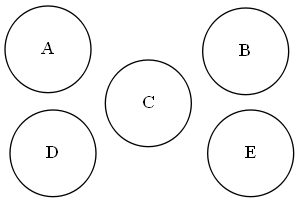
\includegraphics[scale=0.5]{figures/disconnected.png} \hspace{1.4in}} &
\AnswerThreeA
\end{tabular}\\
\end{question}

\vspace{-.2in}
\begin{question}[8]{}\\
\begin{tabular}{cl}
\multirow{1}{*}{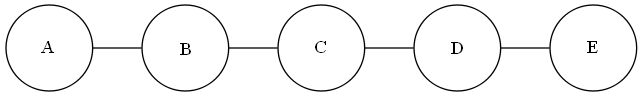
\includegraphics[width=3in]{figures/chain.png}} &
\AnswerThreeB
\end{tabular}\\
\end{question}

\vspace{-.2in}
\begin{question}[8]{}\\
\begin{tabular}{cl}
\multirow{1}{*}{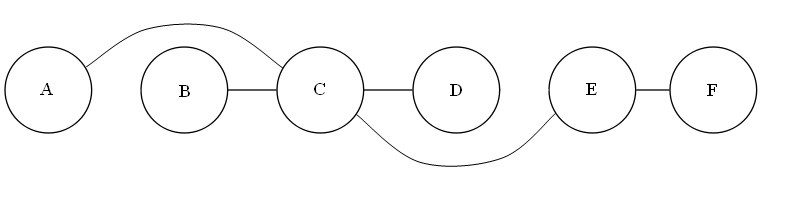
\includegraphics[width=3in]{figures/tree.png}} &
\AnswerThreeC
\end{tabular}
\end{question}

\vspace{-.2in}
\begin{question}[8]{}\\
\begin{tabular}{cl}
\multirow{1}{*}{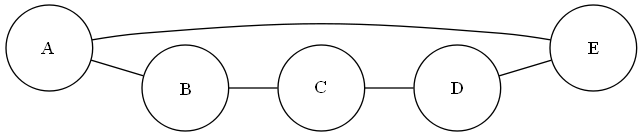
\includegraphics[width=3in]{figures/circle.png}} &
\AnswerThreeD
\end{tabular}
\end{question}

\vspace{-.2in}
\begin{question}[8]{}\\
\begin{tabular}{cl}
\multirow{1}{*}{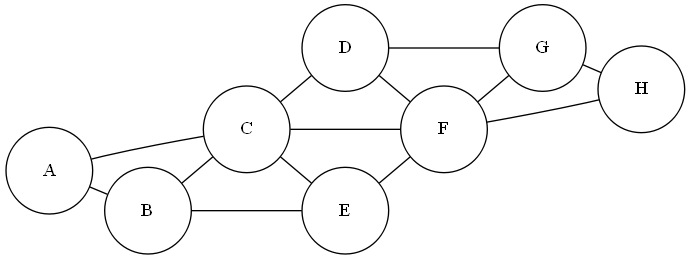
\includegraphics[width=3in]{figures/csp_graph.png}} &
\AnswerThreeE
\end{tabular}
\end{question}

\end{problem}
\newpage
\begin{problem}[10]{Buying a textbook}

Consider a student who has the choice to buy or not buy a textbook for a course. We'll model this as a decision problem with one boolean decision node, B, indicating whether the agent chooses to buy the book, and two Boolean chance nodes, M, indicating whether the student has mastered the material in the book, and P, indicating whether the student passes the course. Of course, there is also a utility node, U. A certain student has an additive utility function: 0 for not buying the book and -100 for buying it; and 2000 for passing the course and 0 for not passing. Sam's conditional probability estimates are as follows:

\hspace{4cm}
\begin{tabular}{ | c | c | c | }
  \hline
  $M$ & $B$ & $P(M|B)$ \\ \hline
  $m$ & $b$ & 0.9 \\ \hline
  $\lnot m$ & $b$ & 0.1 \\ \hline
  $m$ & $\lnot b$ & 0.7 \\ \hline
  $\lnot m$ & $\lnot b$ & 0.3 \\ \hline
\end{tabular}
\hspace{1cm}
\begin{tabular}{ | c | c | c | c | }
  \hline
  $P$ & $M$ & $B$ & $P(P|M,B)$ \\ \hline
  $p$ & $m$ & $b$ & 1.0 \\ \hline
  $\lnot p$ & $m$ & $b$ & 0.0 \\ \hline
  $p$ & $\lnot m$ & $b$ & 0.5 \\ \hline
  $\lnot p$ & $\lnot m$ & $b$ & 0.5 \\ \hline
  $p$ & $m$ & $\lnot b$ & 0.7 \\ \hline
  $\lnot p$ & $m$ & $\lnot b$ & 0.3 \\ \hline
  $p$ & $\lnot m$ & $\lnot b$ & 0.2 \\ \hline
  $\lnot p$ & $\lnot m$ & $\lnot b$ & 0.8 \\ \hline
\end{tabular}
\\

\begin{question}[4] Draw the decision network for this problem. \\
\fbox{\begin{minipage}[t][5cm][t]{17cm}
\FourA
\end{minipage}}
\end{question}

\begin{question}[4] Compute the expected utility of buying the book and of not buying it. \\
\fbox{\begin{minipage}[t][7cm][t]{17cm}
\FourB
\end{minipage}}
\end{question}

{
\renewcommand\truefalsepoints{2}
\begin{truefalse}[\FourC]
Sam should buy the book. TRUE
\end{truefalse}}

\end{problem}
\newpage
\begin{problem}[]{Minimax MDPs}
This exercise considers two-player MDPs that correspond to zero-sum minimax games. Let the players be $A$ and $B$, and let $R(s)$ be the reward for player $A$ in state $s$ (the reward for $B$ is always equal and opposite).

\begin{question}[4]
Let $U_A(s)$ be the utility of state $s$ when it is $A$'s turn to move in $s$, and let $U_B(s)$ be the utility of state $s$ when it is $B$'s turn to move in $s$. All rewards and utilities are calculated from $A$'s point of view (just as in a minimax game tree). Write down Bellman equations defining $U_A(s)$ and $U_B(s)$. \\
\fbox{\begin{minipage}[t][7cm][t]{17cm}
\FiveA
\end{minipage}}
\end{question}
\end{problem}
\newpage

\end{document}